\chapter{Value Analysis} % Main chapter title
\label{chap:valueAnalysis}

Value is the most important concern when it comes to the development of an innovation and/or project. Not only in terms of monetary value, or cost, but specially the value that the product brings to the consumer. 
\par 
According to Lawrence D. Miles, the value of a product or service is attained when measuring the products performance and cost, where the product's performance is its ability to satisfy a certain need \parencite{valueAnalysisAndEngineering}. This means that the value of a product increases when it attains the highest performance at the lowest cost. In mathematics, value can be defined by the following formula:
\par
$$value= \frac{(Performance_x + Capability_x)}{Cost_x}$$
\par

This chapter provides an overview of the value analysis theory that will allow to understand fundamental concepts of this area of research. These concepts are essential to comprehend the value proposition that will also be presented in this chapter.

\section{New Concept Development}
Innovation is not a standard process. It requires a great ability of creativity, opportunity identification and problem solving. The \gls{FFE} is the first stage in that process. This is the point where, in most cases, the opportunities are found and ideas for a solution appears. This stage is a very experimental, unpredictable and unstructured one. As it requires a great amount of creativity, there is no standard process that will lead to a certain result. The results of this will influence the second stage of the process, the \gls{NPD}. This is the process of development and production of a solution to the opportunity that was found. Finally, the product would enter the commercialization phase, where it would be sold to the customers and start generating revenue. However, it was difficult to compare \gls{FFE} practices across different companies. This happens because there is a lack of common terms and definitions for this method's key elements. Without it, it is almost impossible to create new knowledge, or when it was possible, it would be ineffective \parencite{fuzzyFrontEndMethodsToolsThecniques}.
\par
To fill this gap and provide a common language on the front-end activities, Peter Koen and a group of researchers, developed a new theoretical construct, the \gls{NCD} model \parencite{commonLanguageForFFE}. In order to avoid the term \gls{FFE}, as it implies that the activity is mysterious, uncontrollable and unmanageable, Peter Koen introduced a new name for this stage, calling it \gls{FEI} \parencite{managingFrontEndInnovation}. The model is shown in figure \ref{fig:ncdModel}.
\par

\begin{figure}[bh]
\centering
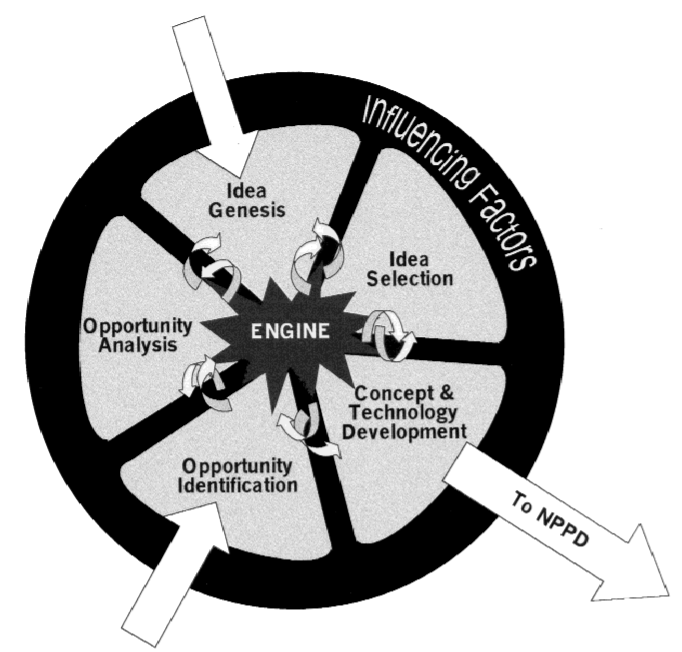
\includegraphics[width=0.8\textwidth,keepaspectratio]{chapters/Value_Analysis/assets/NCD_Model.png}
\caption[NCD model]{NCD model\footnotemark}
\label{fig:ncdModel}
\end{figure}
\footnotetext{retrieved from \url{https://web.stevens.edu/cce/NEW/PDFs/Clarity_FEE.pdf}}

\par
This model is composed by three distinct areas: the engine, at the center, the wheel, which are the five slices near the engine, and the rim, at the border of the model. The engine provides power to the innovation process. It is "fueled by the leadership and culture of the organization" \parencite{commonLanguageForFFE}. The wheel, is composed by five key activity elements: Opportunity Identification, Opportunity Analysis, Idea Generation and Enrichment, Idea Selection and Concept \& Technology Development. The third element, at the border of the model, consists on the external environmental factors that influence the engine and the activity elements. Examples of these factors may be the Business Strategy, Organizational Capabilities, the existent technology to be used and anything that is external to the organization (customers, competitors, trends, etc.). The arrows between the elements are there for the same reason why the model has a circular shape. To indicate that ideas flow and iterate between the five elements. The arrows pointing into the model represent the starting points that a project can have. It may start on either Opportunity Identification, or Idea Genesis. Projects will leave the \gls{FEI} by entering the \gls{NPPD} \parencite{commonLanguageForFFE}.

\subsection{Opportunity Identification and Analysis}
These elements refer, respectively, to the phases where a given company or individual identify an opportunity and analyze it to have a better perception of it and more information regarding the problem. The Opportunity Identification is the most common activity to serve as a starting point for a project, since it reflects a need that is yet to be fulfilled.
\par
It was the case of the project of this dissertation.  As it was already explained in sections \ref{sec:chap1_problem_statement} and \ref{sec:ecommerceAppliedToServices}, despite the existence of multiple online stores selling numerous products, when it comes to services, the number of options decreases drastically, and service providers, are already trying to offer a solution, without technology support. This creates an opportunity to innovate in this sector. Besides that, the existence of a pilot \gls{SP} available to work on the project also took a great part in the opportunity analysis.

\subsection{Idea Genesis and Selection}
The Idea Genesis is the first form of a solution to fulfill the needs found in the Opportunity Identification stage. It includes the process of birth, development and maturation of the opportunity into an concrete idea \parencite{commonLanguageForFFE}. To do this, companies often engage with customers and other companies and institutions in order to understand the real needs of their possible users, and link with cross-functional teams for brainstorming sessions, in order to have a more clear and open view of the whole picture. This element is also a common entry-point for projects. 
\par
In most cases, there are many possible solutions to a certain need. The vastness of good ideas also creates a new problem, which is to choose which ideas the company should select to proceed to the development stage \parencite{commonLanguageForFFE}. This turns out to be a very difficult task, since at this point there is a high degree of uncertainty and the information is very limited. Also, the \gls{ROI} is still a very foggy and risky guess.
\par
In the project in analysis in this thesis, there was already an idea for a solution. The first idea would be to create a solution to suppress the needs of the single pilot client that was already on-board, by developing a website where a customer could order laundry jobs and the \gls{SP} could manage its orders, connecting it to a network of couriers. However, in the first meetings with the student, a new idea surged. The idea was to create a platform, instead of a simple website for just one partner. By being abstracted to the \gls{SP} and the service that was being provided, the platform could easily scale. As the ideas matured, and using the decision process referred in the next sub section, it was decided to proceed with the last one, but taking into account that first partner would be a laundry, and focusing on those needs for the \gls{MVP}.

\subsubsection{Idea Selection using the Analytic Hierarchy Process}
The \gls{AHP}, is a multi-criteria decision method that uses mathematical techniques to aid in the decision makers to choose an option in a group of various alternatives. This process is based in the crossing of the alternatives with the existent criteria \parencite{whatIsAHP}.
\par
In order to select which of the ideas identified in the idea genesis phase, the \gls{AHP} was the method that was used for this. Firstly, an hierarchy decision tree was built:

\begin{figure}[htb]
\centering
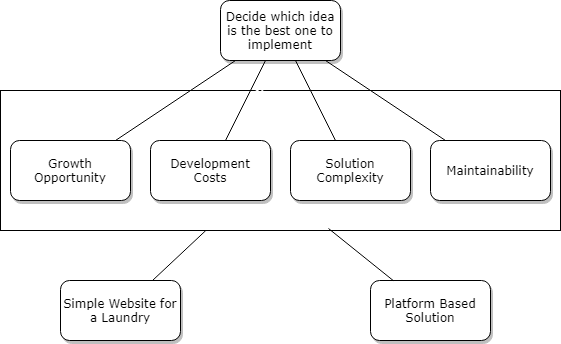
\includegraphics[width=\textwidth,keepaspectratio]{chapters/Value_Analysis/assets/Decision_tree.png}
\caption[Hierarchy Decision Tree]{Hierarchy Decision Tree}
\label{fig:decisionTree}
\end{figure}
\par

The figure \ref{fig:decisionTree} presents the hierarchy decision tree for the idea selection. The first layer reflects the main objectives of this analysis, which is to decide which of the ideas identified in the idea genesis, should be selected. On the second layer, the criteria that will be used for this analysis are presented. These criteria are:
\begin{itemize}
    \item \textbf{Growth Opportunity} - The possibility of the project reaching an higher level and gaining more partners;
    \item \textbf{Development Costs} - The costs in both time and money to develop a given solution;
    \item \textbf{Solution Complexity} - This measures the complexity of a solution for the user. In other words, if it will be difficult to use or not;
    \item \textbf{Maintainability} - This measures how easy, or not, the solution will be to add, remove or correct functionalities to the project.
\end{itemize}
\par

By having these criteria into account, it is possible to evaluate which decision is the best one to accomplish the main objective. The table \ref{tab:ahpEvaluation}


\begin{table}[ht]
\caption{AHP Evaluation Table}
\label{tab:ahpEvaluation}
\resizebox{\textwidth}{!}{%
\begin{tabular}{lllll}
 \textit{Criteria}                  & \textbf{Growth Potential} & \textbf{Development Costs} & \textbf{Solution Complexity} & \textbf{Maintainability}         \\ \cline{2-5} 
\multicolumn{1}{l|}{\textbf{Growth Potential}}    & \multicolumn{1}{l|}{1}    & \multicolumn{1}{l|}{5}     & \multicolumn{1}{l|}{4}       & \multicolumn{1}{l|}{2}           \\ \cline{2-5} 
\multicolumn{1}{l|}{\textbf{Development Costs}}   & \multicolumn{1}{l|}{1/5}  & \multicolumn{1}{l|}{1}     & \multicolumn{1}{l|}{3}       & \multicolumn{1}{l|}{1/2}         \\ \cline{2-5} 
\multicolumn{1}{l|}{\textbf{Solution Complexity}} & \multicolumn{1}{l|}{1/4}  & \multicolumn{1}{l|}{1/3}   & \multicolumn{1}{l|}{1}       & \multicolumn{1}{l|}{12/30}       \\ \cline{2-5} 
\multicolumn{1}{l|}{\textbf{Maintainability}}     & \multicolumn{1}{l|}{1/2}  & \multicolumn{1}{l|}{2}     & \multicolumn{1}{l|}{6}       & \multicolumn{1}{l|}{1}           \\ \cline{2-5} 
\multicolumn{1}{l|}{\textbf{Total}}               & \multicolumn{1}{l|}{2}    & \multicolumn{1}{l|}{8 1/3} & \multicolumn{1}{l|}{14}      & \multicolumn{1}{l|}{3,666666667} \\ \cline{2-5} 
\end{tabular}%
}
\end{table}

The growth opportunity and maintainability are the most important criteria in the decision, since they affect both what the solution can become in the future. The development costs and complexity are, nonetheless, factors to take into account since they can affect the delivery date. However, these last two are not as important as the first ones. 
\par

This matrix presents the normalized matrix in the \gls{AHP} evaluation method.

$M =
\begin{bmatrix}
0,5128 & 0,6000 & 0,2857 & 0,5455 \\
0,1026 & 0,1200 & 0,2143 & 0,1364 \\
0,1282 & 0,0400 & 0,0714 & 0,0455 \\
0,2564 & 0,2400 & 0,4286 & 0,2727 \\
\end{bmatrix}$

\par

Lastly, the table \ref{tab:ahpWeights} presents the weights of each criteria that was used for this decision.
\begin{table}[ht]
\centering
\caption[Weights of each criteria]{Weights of each criteria}
\label{tab:ahpWeights}
\begin{tabular}{ll}
\hline
\multicolumn{1}{|l|}{\textbf{Criteria}} & \multicolumn{1}{l|}{\textbf{Weight}} \\ \hline
Growth Potential                                                & 0,4860                                         \\
Development Costs                                               & 0,1433                                         \\
Solution Complexity                                             & 0,0713                                         \\
Maintainability                                                 & 0,2994                                        
\end{tabular}
\end{table}

\par
Hereupon, taking into account that the growth potential is the most important factor in this decision, the idea of developing a platform instead of a single website directed for a single laundry, was selected to fulfill the needs of this project, since a platform that supports multiple service providers, with different types of services is more likely to grow than a simple website for a laundry.

\subsection{Concept \& Technology Development}
The last element of the \gls{NCD} model is one of the most important. It serves as an exit door to development processes such as the \gls{NPPD}. This activity consists in the "development of a
business case based on estimates of market potential,
customer needs, investment requirements, competitor
assessments, technology unknowns, and overall project
risk" \parencite{commonLanguageForFFE}.
\par
For this project, this phase consisted in the development of the thesis formalization. This document states the problem and objectives of the project, mentioning also several requirements, constraints and restrictions.

\section{Value Proposition}
\label{sec:ValueProposition}
Value Proposition is one of the most widely terms used by companies, nowadays. However, it is difficult to find a clear definition for what it really means. Companies have been defining their \gls{CVP} in many different styles, with their perception of the concept \parencite{valuePropositionBusinessMarkets}. According to this same study, These definitions lie on three major types: all benefits, points of difference and resonating focus.
\begin{itemize}
    \item \textbf{All Benefits}: The most used by managers when asked to build a value proposition. This type simply consists in listing all the benefits that it is believed that the product/solution in question might provide. The more are listed, the better. However, this might lead the customer, to select which product to acquire just based on the price.
    \item \textbf{Points of Difference}: The second approach has the premise that the customer has alternatives other than the product that a given company is offering. As opposed to the previous type, points of difference focuses on the advantage of a product over its competition. It is focused on the question "why should a customer go with our product over our competitors'?" instead of "Why should I buy your product?". From a customer's point of view, this facilitates the process of choosing which is the best solution to his problem.
    \item \textbf{Resonating Focus}: Despite the advantages of the last point over all benefits, there is still room for improvement. The last approach focuses on two points that complement the previous type. This proposition "steadfastly concentrates on the one or two points of difference that deliver, and whose improvement will continue to deliver, the greatest value to target customers" \parencite{valuePropositionBusinessMarkets}. This means that instead of listing all the attributes and benefits of the product, and what differs the product over the competition, resonating focus defends that only the key aspects for the target customers should be mentioned. Secondly, this approach may contain a \gls{PoP}. A \gls{PoP} is a mandatory element for a customer to even consider the company's product as a viable option.
\end{itemize}
\par
Given the possible approaches for the value proposition, for the context of this thesis, it was chosen to follow the last approach, resonating focus. Since for this project, there will be three types of customers, it will be defined, also, three value propositions.

\subsection{Value Proposition for Final Customers}
The final customers are this project's most valuable stakeholder. If the platform doesn't meet the customers' needs, they will not use it, which means that there is no point for service providers to be present in the platform. Eventually, this could lead to the project not being viable.
\par
The value proposition for customers is as it follows:
\par
\begin{itemize}
    \item Choose from a range of service providers;
    \item On-click service request;
    \item Have any goods needed picked-up/delivered at your address, at your time;
    \item Pay with your phone. No need for counting change.
\end{itemize}
\par
Hereupon, the slogan that will be used to attract and present the value proposition to final customers will be:
\par
\textit{Focus on what is important. We take care of the boring tasks.}

\subsection{Value Proposition for Service Providers}
The service providers are the reason why the customers use the platform. Without service providers, there wouldn't be any customers and, by consequence, no business. The value proposition for the service providers is as it follows:
\par
\begin{itemize}
    \item Get online on a ready to use Platform;
    \item Be able to deliver and pickup at customer's address;
    \item Pay what you gain. You only pay fees over the services;
    \item Reduced costs when compared to a proprietary solution;
    \item Increase your range of customers.
\end{itemize}
\par
The slogan that will be used to attract and present the value proposition to service providers will be:
\par
\textit{Do what you do best. The logistics are on us.}

\subsection{Value Proposition for Couriers}
The couriers are the ones with the responsibility of carrying the goods from the customer to the \gls{SP} and vice-versa. It is a very important job since they are the only party to have direct contact to the final customer. The value proposition for couriers is as it follows:
\par
\begin{itemize}
    \item Flexible work hours;
    \item Be your own boss;
    \item Easy to get on-board;
    \item No usage costs;
    \item Increase your income.
\end{itemize}
\par
With this, the slogan that will be used to attract and present the value proposition to couriers will be:
\par
\textit{Create your own schedule and increase your income}

\section{Value for the Customer}
When developing a new product or service, one of the most important things that companies must have in mind, is the value that it will bring to their customers. However, this exercise is a harder task than it appears. The reason for this is because value is a subjective concept. It is a trade-off between benefits and sacrifices. Those benefits and sacrifices might have a different impact on distinct customer segments. What might be one's benefit, might be indifferent for other. Even if we look to the individual customer in a single segment, this phenomenon may occur due to the individuality of each customer. Nevertheless, it is expected to occur less often. Value may also be relative to the current competition on the market. When a certain company launches a product that has similar functions to a competitor's early released product, the customers are already used to that features, which makes it lose the novelty factor \parencite{relationshipValueAndRelationshipQuality}.
\par
\gls{VC} is described by Tony Woodall as 
\say{any demand-side, personal perception of advantage arising out of a customer’s association with an organization’s offering, and can occur as reduction in sacrifice; presence of benefit (perceived as either attributes or outcomes); the resultant of any weighed combination of sacrifice and benefit (determined and expressed either rationally or intuitively); or an aggregation, over time, of any or all of these} \parencite{conceptualisingValueForTheCustomer}. On this same study, Woodall divides \gls{VC} into two sub-forms: Nature of Derived \gls{VC} and Contingent \gls{VC}. The first one refers to \gls{VC} in its derived form. It focuses on excellence and more in derivatives as material value, functional value and emotional value. It is also called "Consumption Value" \parencite{weAreWhatWeBuy}. Most of these are types of value don't change over the time. The second one, focuses on the value on a longitudinal timeline, from the period before the customer buys the product, passing for the transaction it-self and ending in the after use. The whole process is part of the experience in Contingent \gls{VC}. 
\par

\begin{figure}[htb]
\centering
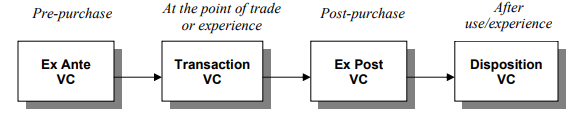
\includegraphics[width=\textwidth,keepaspectratio]{chapters/Value_Analysis/assets/contigent-value-phases.png}
\caption[Longitudinal Perspective on \gls{VC}]{A Longitudinal Perspective on \gls{VC}\footnotemark}
\label{fig:longitudinalVC}
\end{figure}
\footnotetext{retrieved from \url{https://cdn.ymaws.com/www.ams-web.org/resource/resmgr/original_amsr/woodall12-2003.pdf}}

\par
In the figure \ref{fig:longitudinalVC}, it is possible to verify each of the temporal phases inherent to the Contingent \gls{VC}. Each of these temporal stages have associated values, benefits and sacrifices. 
\par
The table \ref{tab:contingentVCMapping} presents a mapping between each of the temporal phases of the Contingent \gls{VC}, and some of its associated values, benefits and sacrifices, for the project in analysis in this thesis. As was already exposed in exposed in section \ref{sec:ValueProposition}, there are three different clients of this system: the final customer, the service provider, and the courier. Since the main problem to be solved by this project will be a problem of the service providers, the mapping was done for the benefits and sacrifices of that specific client. 
\par
Focusing on the benefits and the sacrifices, it is verified that there are many benefits for the customer and just a few sacrifices, most of them related to the price and training costs.
\par
\begin{table}[ht]
\centering
\caption{Contingent VC Temporal Stages Values mapping}
\begin{tabular}{|l|lll} 
\hline
\textbf{Temporal Stage}~ & \multicolumn{1}{l|}{\textbf{Values}}                                                                      & \multicolumn{1}{l|}{\textbf{Benefits}}                                                                             & \multicolumn{1}{l|}{\textbf{Sacrifices}}                                               \\ 
\hline
Ex Ante VC      & \begin{tabular}[c]{@{}l@{}}Expected value\\Desired value\end{tabular}                            & \begin{tabular}[c]{@{}l@{}}Product characteristics\\Features~ ~\end{tabular}                              & Price                                                                         \\ 
\cline{1-1}
Transaction VC  & \begin{tabular}[c]{@{}l@{}}Transaction value\\Exchange value \\Acquisition value~ ~\end{tabular} & \begin{tabular}[c]{@{}l@{}}Support\\Security~ ~\end{tabular}                                              & Acquisition costs                                                             \\ 
\cline{1-1}
Ex Post VC      & \begin{tabular}[c]{@{}l@{}}Delivered value\\Received value \\Postpurchase value\end{tabular}     & \begin{tabular}[c]{@{}l@{}}Functional benefits~\\Operational benefits\\Logistical benefits~~\end{tabular} & \begin{tabular}[c]{@{}l@{}}Training Costs\\Installation costs~~\end{tabular}  \\ 
\cline{1-1}
Disposition VC  & \begin{tabular}[c]{@{}l@{}}Use value\\Redemption value~ ~\end{tabular}                           & \begin{tabular}[c]{@{}l@{}}Service support\\Reliability\\Convenience\\\end{tabular}                       & Maintenance costs                                                             \\
\cline{1-1}
\end{tabular}
\label{tab:contingentVCMapping}
\end{table}

\par
The Ex Ante and Ex Post perceptions of a product will prepare the customer for the experience that he/she will have during this process. They will both take part in the customer perception of the quality of the service. In the case of the first temporal stage, it will affect the customer's perception of the service/product's value. The perceived value is the impression that is passed to the possible customer of the value of what is being presented. However, this process depends a lot in the customer's previous experiences and expectations \parencite{perceivedValue}.

